\documentclass[10pt]{report}
\usepackage[utf8]{inputenc}
\usepackage{graphicx}
\usepackage[backend=biber]{biblatex}
\usepackage{ulem}
\bibliography{biblio}
\nocite{*} 
\setlength{\parindent}{0pt}

\title{\textbf{Proyecto Final}}
\author{Integrantes:\\
Luis Alfonso Bravo Flores\\
Gonzalez Lopez Roberto Alejandro\\
Navarro Osorio Armando\\
Cruz Galván Alberto Israel} % Replace Me with your name!
\date{26/Mayo/2020}

\begin{document}

\maketitle

%%%%%%%%%%%%%%%%%%%%%%%%%%%%%%%%%%%%%%%%%%%%%%%%%%%%%%%%%%%%%%%%%%%%%%%%%%%%%%



\chapter*{Introducción}

El proyecto final consistió en crear una base de datos de una papelería que buscaba innovar la manera en que almacenará su información y que tuviera los siguientes requerimientos:\\

Se deseaba tener almacenados datos como la razón social, domicilio, nombre
y teléfonos de los proveedores, razon social, nombre, domicilio y al menos un
email de los clientes. Se necesitaba tener un inventario de los productos que se
venden, en el que debe guardarse el código de barras, precio al que fue comprado
el producto, fecha de compra y cantidad de ejemplares en la bodega (stock).
Se deseaban guardar la marca, descripcion y precio de los regalos, artculos de
papelera, impresiones y recargas, siempre y cuando se tenga su correspondiente
registro en el inventario. Se debían también guardarse el número de venta, fecha de
venta y la cantidad total a pagar de la venta, así como la cantidad de cada
artículo y precio total a pagar por artículo. \\

Además, se requería que:

\begin{itemize}

\item Al recibir el código de barras de un producto, se regresará la utilidad.

\item Cada que haya la venta de un artculo, se debía decrementar el stock por
la cantidad vendida de ese artículo. Si el valor llegaba a cero, se abortaba la
transacción. Si hay menos de 3, se emitía un mensaje.

\item Dada una fecha, o una fecha de inicio y fecha de n, se regresaba la cantidad total que se vendió en esa fecha/periodo.

\item Se obtuviera el nombre de aquellos productos de los cuales hay menos de 3 en stock. De manera automática se generará una vista que contenga información necesaria para asemejarse a una factura de una compra.

\item Se creará al menos, un índice, del tipo que se prefiera y donde se prefiera. 

\end{itemize}


\chapter*{Plan de Trabajo}

\begin{enumerate}
    \item La primera actividad del proyecto consistió en analizar detalladamente el problema presentado, para ello fue necesario que cada integrante del equipo diera su punto de vista de cual modelo entidad relación fuera el correcto, para así construirlo conjuntamente. Se definieron así tanto las entidades como los atributos y las relaciones correspondientes con cada uno de ellos. Finalmente con el diseño construido, el siguiente paso fue construir el modelo relacional que definiría las tablas de nuestra base de datos.
    
    \item La siguiente actividad consistio en conformar el Development team que se encargaría de la programación del proyecto. Esté se conformo de la siguiente manera:
    
        \begin{enumerate}
            \item Alberto tomo el rol de desarrollo del backend que consistio en la programación en PostgresSQL de las relaciones propuestas así como de las funciones que serían utilizadas en la creación del proyecto.
            \item Alejandro tomo el rol de desarrollo del Frontend que concierne a la conexión entre la base de datos y la página web, así como la programación de la interfaz gráfica.
            \item Alfonso tomo el rol de desarrollador de la documentación en LATEX así como la integración de cada una de las partes del proyecto.
        \end{enumerate}
    
    \item La última actividad del proyecto  consistió en juntar cada una de las partes del proyecto y hacer las pruebas correspondietes de su funcionamiento. 



\end{enumerate}


\chapter*{Diseño}
\setlength{\parskip}{-5mm}
Como todo diseño, existen pasos a desarrollar y, lo dividiremos en tres fases: 

\begin{enumerate}
    \item \textbf{Diseño conceptual}
    \item \textbf{Diseño lógico }
    \item \textbf{Diseño físico}\\ \\
\end{enumerate}

\textbf{El Diseño Conceptual}\\
\setlength{\parskip}{10mm}
Para conseguir alcanzar el objetivo planteado, como equipo, primeramente definiremos la estructura de los datos que deben de tener nuestro sistema de información. 
Consistirá describir a alto nivel  la estructura que tendrá nuestra base de datos. En él, se describió la información al almacenar en nuestro destino final, quye es nuestra base de datos llamada \textbf{PROYECTO\_PAPELERIA}. 
    
    \begin{figure}[htb]
    \centering
    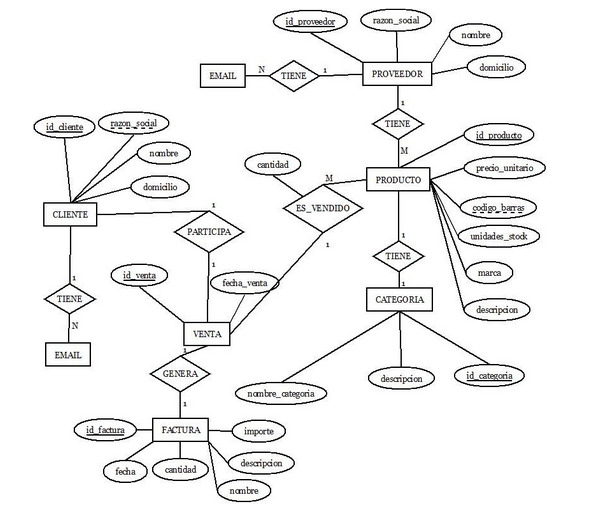
\includegraphics[width=0.8\linewidth]{DER.png}
    \caption{Diagrama Entidad - Relación}
    \end{figure}

\textbf{El Diseño lógico\\ \\}
\setlength{\parskip}{0mm}
Una vez obtenido el modelo entidad relación (MER), se comienza a crear, a partir de él, el modelo relacional (MR). Comenzamos replicando las entidades a tablas y los atributos de las entidades, fueron sustituidos por campos en dichas tablas, respetando, por obviedad, las claves primarias.

Se analizaron cada una de las relaciones que hubiera en el MER, se convirtieron a tablas y, se propagaron las llaves foráneas correspondientes.


\begin{flushleft} \ttfamily
\setlength{\parskip}{0mm}

CATEGORIA{[id\_categoria](PK),nombre\_categoria, descripcion}\\ --TABLA\_1\\

PROVEEDORES{[id\_proveedor](PK),razon\_social, domicilio,nombre}\\ --TABLA\_2\\

TELEFONO\_PROVEEDORES{[id\_proveedor(FK),telefono](PK)} --TABLA\_3\\

PRODUCTOS{[id\_producto,id\_precio\_unitario,codigo\_barras](PK),
[id\_categoria,id\_proveedor](FK),unidades\_stock,marca,\\
descripcion}--TABLA\_4\\

CLIENTES{[id\_cliente (PK)],razon\_social,nombre,domicilio}\\ --TABLA\_5

EMAIL\_CLIENTES{[id\_cliente, email](PK)} --TABLA\_6\\

VENTAS{[id\_venta (PK)],id\_cliente (FK), fecha\_venta} --TABLA\_7\\

VENTA\_DETALLES{[id\_venta (PK)](FK),id\_producto(FK),\\ precio\_unitario(FK),cantidad} --TABLA\_8\\
VENTA\_DETALLES{[id\_factura(PK)],id\_venta(FK),razon\_social,\\
fecha,cantidad,nombre,desdescripcion,importe} --TABLA\_9\\


\end{flushleft}

 
    
   \begin{figure}[htb]
    \centering
    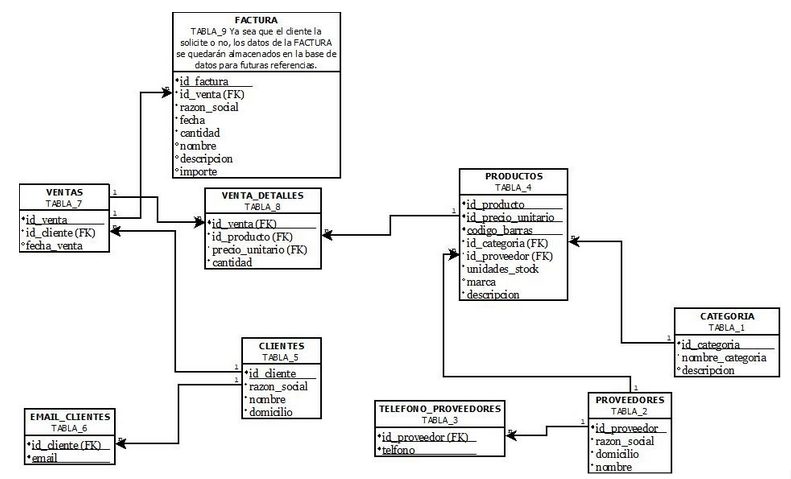
\includegraphics[width=0.9\linewidth]{MER.png}
    \caption{Modelo Entidad Relación}
    \end{figure}


\textbf{\\El Diseño físico\\}
\setlength{\parskip}{0mm}
Evidentemente, el diseño físico, varía ligeramente de acuerdo al sistema generador de base de datos. El objetivo, será implementar físicamente  (en memoria del servidor), del diseño lógico que se ha implementado, esto, con ayuda del lenguaje de consulta estructurado \textbf{SQL}. 






     El siguiente paso consistio en hacer el desarrollo, el cual lo dividimos en dos partes:\\ \\
    
    {\textbf{BACKEND}} \\
    
    {\large{\textsc {En la parte del servidor se crearon la base de
    datos, las tablas y se insertaròn los datos correspondientes. Primeramanete se creo la base de datos:}}}
    
            \begin{flushleft} \ttfamily
            ---------------------------------------------------------------------\\
            --AUTORES: solucionesTI\_AAAA\\
            --BD:PROYECTO\_2020 \\
            --DESCRIPCIÒN: CREACIÒN DE LA BASE DE DATOS\\
            --FECHA DE CREACIÒN \\
            ---------------------------------------------------------------------\\
            CREATE DATABASE "PROYECTO\_PAPELERIA"\\
            WITH \\
            OWNER = postgres\\
            ENCODING = 'UTF8'\\
            CONNECTION LIMIT = -1;\\
            \end{flushleft} 
            
            
 {\large{\textsc{\\La siguiente parte fue crear cada una de las tablas, con sus respectivas llaves, tanto primarias como foraneas, constrains, tipos de datos, etc. Lo anterior lo hicimos con la siguiente función:\\}}}
  
    \begin{flushleft} \ttfamily 

   CREATE OR REPLACE FUNCTION fn\_diseño\_fisico() RETURNS VOID
    LANGUAGE SQL\\
    AS\\
    \$\$\\
	--===========================================================\\
	--AUTORES: solucionesTI\_AAAA\\
	--BD:PROYECTO\_PAPELERIA\\
	--DESCRIPCIÓN: Diseño físico de la base de datos.\\
	--FECHA DECREACIÓN \\
	--============================================================\\

	---------------------------------------------------------------------\\
	CREATE TABLE CATEGORIA ( --TABLA\_1\\
		 id\_categoria	  INT GENERATED ALWAYS AS IDENTITY NOT NULL\\
		,nombre\_categoria VARCHAR(60)		NOT NULL\\
		,descripcion      VARCHAR(100) \\
		,CONSTRAINT PK\_CATEGORIA PRIMARY KEY(id\_categoria)\\
	);\\
	---------------------------------------------------------------------\\
	CREATE TABLE PROVEEDORES(--TABLA\_2\\
		 id\_proveedor INT GENERATED ALWAYS AS IDENTITY NOT NULL\\
		,razon\_social VARCHAR(100)		NOT NULL\\
		,domicilio	  VARCHAR(300)		NOT NULL\\
		,nombre		  VARCHAR(100)		NOT NULL\\
		,CONSTRAINT PK\_PROVEEDORES PRIMARY KEY(id\_proveedor)\\
	);\\
	---------------------------------------------------------------------\\
	CREATE TABLE TELEFONO\_PROVEEDORES(--TABLA\_3\\
		 id\_proveedor INT				NOT NULL\\
		,telefono	  VARCHAR(48)		NOT NULL\\
		,CONSTRAINT PK\_TELEFONO\_PROVEEDORES PRIMARY\\ KEY(id\_proveedor,telefono)\\
		,CONSTRAINT FK\_TELEFONO\_PROOVEDORES FOREIGN\\ KEY(id\_proveedor)\\
		 REFERENCES PROVEEDORES(id\_proveedor)\\
	);\\
	---------------------------------------------------------------------\\
	CREATE TABLE PRODUCTOS( --TABLA\_4\\
		 id\_producto        INT GENERATED ALWAYS AS IDENTITY NOT\\ NULL\\
		,nombre\_producto	VARCHAR(50)		  NOT NULL\\		
		,precio\_unitario 	DECIMAL	 		  NOT NULL\\	
		,id\_categoria       INT				  NOT NULL\\
		,id\_proveedor       INT               NOT NULL\\
		,codigo\_barras 	    VARCHAR(100)	  NOT NULL\\
		,unidades\_stock     INT 	 		  NOT NULL\\
		,marca		        VARCHAR(50)  --PUEDE SER NULL\\
		,descripcion	    VARCHAR(100) --PUEDE SER NULL\\
		,CONSTRAINT PK\_PRODUCTOS PRIMARY\\ KEY(id\_producto,precio\_unitario)\\
		,CONSTRAINT FK\_PRODUCTOS\_CATEGORIA FOREIGN\\ KEY(id\_categoria)\\
		REFERENCES CATEGORIA(id\_categoria)\\
		,CONSTRAINT FK\_PRODUCTOS\_PROVEEDORES FOREIGN\\ KEY(id\_proveedor)\\
		REFERENCES PROVEEDORES(id\_proveedor)\\
	);\\
	---------------------------------------------------------------------\\
	CREATE TABLE CLIENTES(--TABLA\_5\\
		 id\_cliente   INT GENERATED ALWAYS AS IDENTITY NOT NULL\\
		,razon\_social VARCHAR(100)		NOT NULL\\
		,domicilio    VARCHAR(300)		NOT NULL\\
		,nombre		  VARCHAR(100)		NOT NULL\\	  
		,CONSTRAINT PK\_CLIENTE PRIMARY KEY(id\_cliente)\\
	);\\
	---------------------------------------------------------------------\\
	CREATE TABLE EMAIL\_CLIENTES(--TABLA\_6\\
		 id\_cliente INT			NOT NULL\\
		,email		VARCHAR(50)	NOT NULL\\
		,CONSTRAINT PK\_EMAIL\_LIENTES PRIMARY KEY(id\_cliente,email)\\
		,CONSTRAINT FK\_EMAIL\_CLIENTES FOREIGN KEY(id\_cliente)\\
		REFERENCES CLIENTES(id\_cliente)\\
	);\\
	---------------------------------------------------------------------\\
	CREATE TABLE VENTAS(--TABLA\_7\\
		 id\_venta    VARCHAR(50)	    NOT NULL\\
		,id\_cliente  INT				NOT NULL\\
		,fecha\_venta DATE NOT NULL\\
		,CONSTRAINT PK\_VENTAS PRIMARY KEY(id\_venta)\\
		,CONSTRAINT FK\_VENTAS\_CLIENTES FOREIGN KEY(id\_cliente)\\
		REFERENCES CLIENTES(id\_cliente)\\
	);\\
	---------------------------------------------------------------------\\
	CREATE TABLE VENTA\_DETALLES(--TABLA\_8\\
		 id\_venta 	        VARCHAR(50)   NOT NULL\\
		,id\_producto 	    INT			  NOT NULL\\
		,precio\_unitario 	DECIMAL		  NOT NULL\\
		,cantidad			INT			  NOT NULL\\
		,CONSTRAINT PK\_VENTA\_DETALLES PRIMARY KEY(id\_venta)\\
		,CONSTRAINT FK\_VENTA\_DETALLES\_VENTAS FOREIGN\\ KEY(id\_venta)\\
		REFERENCES VENTAS(id\_venta)\\
		,CONSTRAINT FK\_VENTA\_DETALLES\_PRODUCTOS FOREIGN\\ KEY(id\_producto,precio\_unitario)\\
		REFERENCES PRODUCTOS(id\_producto,precio\_unitario)\\
	);\\
	---------------------------------------------------------------------\\
\$\$;
    
     \end{flushleft} 
    
    
   {\large{\textsc{ \\La siguiente parte fue insertar los datos utilizados a cada una de nuestras tablas. Igual que en el paso anterior, hicimos las insercciones mediante una función:\\}}}
        
    
    \begin{flushleft} \ttfamily
    
    CREATE OR REPLACE FUNCTION fn\_inserta\_datos() RETURNS VOID
    LANGUAGE SQL\\
    AS
    \$\$
	--===========================================================\\
	--AUTORES: solucionesTI\_AAAA
	--BD:PROYECTO\_PAPELERIA
	--DESCRIPCIÓN:Insercion de datos.
	--FECHA DECREACIÓN 
	--============================================================\\

	--------------------------------------------------------------\\
	--TABLA\_1 CATEGORIA\\
	INSERT INTO CATEGORIA(nombre\_categoria,descripcion)\\
	VALUES('Papeleria','Articulos escolares y de oficina');\\
	INSERT INTO CATEGORIA(nombre\_categoria,descripcion)\\ 
	VALUES('Regalos','Articulos relacionados a regalos (regalos y\\ envolturas)');\\
	INSERT INTO CATEGORIA(nombre\_categoria,descripcion)\\
	VALUES('Servicio de impresiones','Imp. B/N, color y en\\ diferentes tamaños');\\
	INSERT INTO CATEGORIA(nombre\_categoria,descripcion)\\
	VALUES('Servicio de recargas','Recargas telefónicas a \\
	todas las compañias');\\
	--SELECT * FROM CATEGORIA;\\
	--------------------------------------------------------------\\
	--TABLA\_2 PROVEEDORES(ATRIBUTO DOMICILIO COMO\\ Estado|C.P.|Col.|Calle y No.|nombre)\\
	INSERT INTO PROVEEDORES(razon\_social,domicilio,nombre)\\
	VALUES('Papeleria\_Mesones','CDMX, 06080, Centro, Mesones\\ 32','Papeleria Mesones');\\
	INSERT INTO PROVEEDORES(razon\_social,domicilio,nombre)\\
	VALUES('Tony\_Superpapeleria\_Mesones','CDMX, 06090, Centro,\\ Mesones 160-B','Tony Superpapeleria Mesones');\\
	INSERT INTO PROVEEDORES(razon\_social,domicilio,nombre)\\
	VALUES('La\_Reyna\_De\_Mesones\_SA\_de\_CV','CDMX, 06090,\\ Centro, Jesús María 118','La Reyna');\\
	INSERT INTO PROVEEDORES(razon\_social,domicilio,nombre)\\
	VALUES('Mobil\_Mex\_SA\_de\_CV,','CDMX, 11570, Lomas de\\ Chapultepec, Monte Elbruz 132','Mobil Mex');\\
	INSERT INTO PROVEEDORES(razon\_social,domicilio,nombre)\\
	VALUES('Grupo\_Fila Dixon','EDOMEX, 54940, Tultitlan,Autopista\\ Mexico-Queretaro 104 Int C','Grupo Dixon');\\
	INSERT INTO PROVEEDORES(razon\_social,domicilio,nombre)\\
	VALUES('Papel\_S.A.','CDMX, 06720, Doctores, Doctor Andrade\\ 78','Papeles en tamaños');\\
	INSERT INTO PROVEEDORES(razon\_social,domicilio,nombre)\\
	VALUES('Fantasías\_Miguel\_SA\_de\_CV','EDOMEX, 53100, \\
	Satelite, Cto Cirujanos 5','Fantasías Miguel');\\
	INSERT INTO PROVEEDORES(razon\_social,domicilio,nombre)\\
	VALUES('Comercializadora\_de\_impresoras\_Angel\_SA\_CV',\\
	'CDMX, 06090,Centro,Mesones 55, Papeleria\\ Mesones','Angel\_impresoras');\\
	--SELECT * FROM PROVEEDORES;\\
	
                    .\\
                    .\\
                    .\\
                    .\\
                    .\\
                    .\\
                    .\\
                    .\\
  
    \end{flushleft}
    
    {\textbf{FRONTEND}} \\




\chapter*{Implementación}

\textbf{REQUERIMIENTOS}

\begin{enumerate}
    \item Al recibir el código de barras de un producto, regrese la utilidad.
    
    \begin{flushleft} \ttfamily
    CREATE OR REPLACE FUNCTION fn\_utilidad(ps\_codigo\_barras VARCHAR(50))
    RETURNS NUMERIC LANGUAGE plpgsql
    --==========================================================
    --AUTORES: solucionesTI\_AAAA
    --BD:PROYECTO\_PAPELERIA
    --DESCRIPCIÓN: Función que retorna la utilidad de un producto\\ al recibir el código de barras
    --FECHA DE CREACIÓN 
    --==========================================================
    AS \$\$\\
    DECLARE\\
	    tprecio\_venta 	  NUMERIC;\\
		costo\_adquisicion NUMERIC;\\
		utilidad 		  NUMERIC;\\
		ganancia		  NUMERIC;\\
    BEGIN\\
	    SELECT precio\_unitario\\
	    FROM PRODUCTOS\\
	    WHERE codigo\_barras=ps\_codigo\_barras\\
	    INTO precio\_venta; --Obtenemos el precio de venta del\\ producto deseado (del catálogo).\\
	
	    SELECT 0.30*precio\_venta\\
	    INTO ganancia; --Obtenemos la ganancia del articulo.\\
	
	    costo\_adquisicion:=precio\_venta-ganancia;--costo\_\\
	    adquisicion=precio\_venta-ganancia.\\
	    utilidad:=precio\_venta-costo\_adquisicion;--Utilidad es\\ resultado de esta resta.\\
	
	    RETURN utilidad;\\
    END\\
    --SELECT fn\_utilidad('A-0100-R') Ejemplo de invocación de la\\ utilidad de la pluma.\\
    --select * from productos;Para ver el catálogo.\\
    \$\$;\\
    
    \end{flushleft}
    
    \item Cada que haya la venta de un artículo, debería decrementarse el stock por la cantidad vendida de ese artículo. Si el valor llega a cero, abortar la transacción. Si hay menos de 3, emitir un mensaje.
    
    \begin{flushleft} \ttfamily
    CREATE OR REPLACE FUNCTION stock()\\
    RETURNS trigger AS \$\$\\
    BEGIN\\
	  IF unidades\_stock<=0 THEN \\
		ROLLBACK;\\	  
		RAISE NOTICE 'No hay productos en almacen';\\
	  ELSE \\
	  	--BEGIN\\
		UPDATE productos SET\\
      	unidades\_stock=unidades\_stock-cantidad\\
      	WHERE productos.precio\_unitario=venta\_detalles.\\
      	precio\_unitario and\\ 
		productos.id\_producto=venta\_detalles.id\_producto;\\
		--COMMIT\\
				IF unidades\_stock<0 THEN\\
					ROLLBACK;\\
					RAISE NOTICE 'No se puede hacer la venta';\\
				ELSIF unidades\_stock<3 THEN \\
					RAISE NOTICE 'Hay menos de 3 productos en\\ almacen';\\
				END IF;\\
       END IF;\\
--RETURN NULL;\\
END\\

\$\$ LANGUAGE plpgsql;\\ 

CREATE TRIGGER stock\\
  BEFORE INSERT\\
  ON VENTA\_DETALLES\\
  FOR EACH ROW\\
  EXECUTE PROCEDURE stock();\\

    \end{flushleft}
    
    
    
    
    \item Dada una fecha, o una fecha de inicio y fecha de fin, regresar la cantidad total que se vendió en esa fecha/periodo.
    
    \begin{flushleft} \ttfamily
    --============================================================\\
    --AUTORES: solucionesTI\_AAAA\\
    --BD:PROYECTO\_PAPELERIA\\
    --DESCRIPCIÓN: Dada una fecha de inicio y una fecha de fin,\\ regresar la cantidad total que se vendió en esa fecha/periodo.\\ 
   ==============================================================\\
    DECLARE\\
            ln\_total\_vendido\_por\_periodo NUMERIC :=0;\\
		    ld\_fecha\_inicio   DATE:=to\_date(ps\_fecha\_\\
		    inicio,'YYYYMMDD');\\
		    ld\_fecha\_fin      DATE:=to\_date(ps\_fecha\_\\
		    fin,'YYYYMMDD');\\
    BEGIN\\
	        SELECT SUM (precio\_unitario*cantidad)\\ 
	        FROM VENTA\_DETALLES VD\\
		    INNER JOIN VENTAS V on V.id\_venta=VD.id\_venta\\ 
	        WHERE V.fecha\_venta BETWEEN ld\_fecha\_inicio AND\\ ld\_fecha\_fin\\
	        INTO ln\_total\_vendido\_por\_periodo;\\
	        --Mediante esta consulta, se obtienen \\
	        --la cantidad de dinero vendido en el periodo\\ solicitado.\\
	
	        RETURN ln\_total\_vendido\_por\_periodo;\\
            --select\\ public.fn\_cantidad\_total\_vendida\_por\_periodo\\
            ('20200507','20200507');\\
    END\\
    \$\$;\\

    \end{flushleft}
    
    \item   Permitir obtener el nombre de aquellos productos de los cuales hay menos de 3 en stock.
    
    \begin{flushleft} \ttfamily
    CREATE VIEW vw\_articulos\_por\_agotarse
    AS\\
    --==========================================================\\
    --AUTORES: solucionesTI\_AAAA\\
    --BD:PROYECTO\_PAPELERIA\\
    --DESCRIPCIÓN: Obtención de productos que estén por agotarse,\\
    es decir, aquellos productos cuyas unidades en stock sean\\ menores a 3.\\
    --LLAMADO: SELECT * FROM vw\_articulos\_por\_agotarse
    --===========================================================\\
	SELECT nombre\_producto,descripcion\\ 
	FROM PRODUCTOS\\
	WHERE unidades\_stock <=2 AND unidades\_stock>0;\\
    \end{flushleft}
    
    \item De manera automática se genere una vista que contenga información necesaria para asemejarse a una factura de una compra.
    
    \begin{flushleft} \ttfamily
    CREATE OR REPLACE FUNCTION fn\_genera\_factura()\\
    RETURNS TRIGGER LANGUAGE plpgsql\\
    --==========================================================\\
    --AUTORES: solucionesTI\_AAAA\\
    --BD:PROYECTO\_PAPELERIA\\
    --DESCRIPCIÓN: Genera datos de factura, de forma automática \\
    al generar una venta.\\
    --FECHA DE CREACIÓN \\
    --===========================================================\\
    AS\\
    \$\$
    DECLARE\\ 
        li\_id\_venta 		VARCHAR(50);\\
		ls\_razon\_social 	VARCHAR(100);\\
		ld\_fecha\_date		DATE:=current\_date;\\
		li\_cantidad			INT:=0;\\
		ls\_nombre\_producto  VARCHAR(50);\\
		ls\_descripcion		VARCHAR(100);\\
		li\_importe			NUMERIC;\\
    
    BEGIN\\
	li\_id\_venta:=new.id\_venta;\\
	--------------------------------------------------------------\\
	SELECT razon\_social\\
	FROM CLIENTES Cte\\
	INNER JOIN VENTAS V 		 ON V.id\_cliente=Cte.id\_cliente\\
	INNER JOIN VENTA\_DETALLES VD ON VD.id\_venta=V.id\_venta\\
	WHERE VD.id\_venta=new.id\_venta\\ 
	INTO ls\_razon\_social;--Obtenemos la razon social del cliente\\ que compra.\\
	--------------------------------------------------------------\\
	li\_cantidad:=new.cantidad;\\
	--------------------------------------------------------------\\
	SELECT nombre\_producto\\
	FROM PRODUCTOS\\
	WHERE id\_producto=new.id\_producto\\
	INTO ls\_nombre\_producto;\\
	--------------------------------------------------------------\\
	SELECT descripcion\\
	FROM PRODUCTOS\\
	WHERE id\_producto=new.id\_producto\\
	INTO ls\_descripcion;\\
	--------------------------------------------------------------\\
	li\_importe:=new.cantidad*new.precio\_unitario;
	--------------------------------------------------------------\\
	
	INSERT INTO FACTURA(id\_venta,razon\_social,fecha,cantidad,\\
	nombre\_producto,descripcion,importe)\\
	VALUES(li\_id\_venta,ls\_razon\_social,ld\_fecha\_date,\\
	li\_cantidad,ls\_nombre\_producto,ls\_descripcion,li\_importe);\\
	
	return new;\\
    END
    \$\$;\\
    
   CREATE TRIGGER tr\_crea\_factura AFTER INSERT on VENTA\_\\
    DETALLES FOR EACH ROW\\
    EXECUTE PROCEDURE fn\_genera\_factura()\\
    \end{flushleft}
  
    
    
\end{enumerate}


\chapter*{Presentación}
\chapter*{Conclusiones}

\begin{enumerate}
    \item \textbf{Luis Alfonso Bravo Flores:} Los objetivos del curso se cumplieron con este proyecto, ya que pusimos en práctica todo lo visto en clase. El proyecto fue un reto importante ya que enfrentamos dificultades de operación puesto que nos tuvimos que comunicar en linea por el problema de la pandemia. Cada uno de los integrantes aportó deacuerdo a sus habilidades para que este proyecto se construyera. Nos llevamos una buena experiencia para futuros proyectos.
    \item \textbf{Cruz Galván Alberto Israel:} sin lugar a dudas la realización de este proyecto, conjugó un reto en múltiples sentidos. Desde la capacidad de trabajo en equipo, organización, delegar responsabilidades, también, poner a prueba nuestros conocimientos adquiridos a lo largo del semestre de la asignatura y desde luego, nuestras capacidades como ingenieros para resolver problemas.Durante el desarrollo del proyecto, se tuvo que llevar a la práctica la teoría del diseño de la base de datos, desde la parte del diseño, entendiendo los requerimientos del problema para que conjuntamente, se plantearan y se resolvieran en equipo de la mejor manera posible. El trabajo en equipo y la organización son inherentes a cualquier ramo ingenieril.  
    \item \textbf{Gonzalez Lopez Roberto Alejandro:} Este proyecto me demostro la importancia del manejo de tiempo y de personas. Ademas de la importancia del trabajo de investigacion, ya que se dieron problemas con la interfaz grafica que no se tenian contempladas y otros problemas con la base de datos con las especificaciones. Aun asi solo queda aprender de este proyecto y aplicarlo a futuros.
    \item \textbf{Navarro Osorio Armando:}Con el desarrollo de este proyecto se adquirieron nuevos conocimientos así como nuevas habilidades, las cuales son muy usadas en la vida profesional. La que más cabe mencionar fue el trabajo en equipo ya que se tiene que tener un buena bitácora para desarrollar cada uno de los puntos en tiempo y forma.  Fue un proyecto en donde se puso en juego nuestra propia disciplina así como el uso de ser autodidactas en la parte de la base de datos.

\end{enumerate}


\printbibliography

\end{document}
